\documentclass[12pt]{article}
\usepackage[a4paper, total={5.5in, 9in}]{geometry}
\usepackage{amsmath}
\usepackage{pgfplots}
\pgfplotsset{compat=1.18}
\usepackage{amsfonts}
\usepackage{graphicx}
\usepackage{enumitem}
\usepackage{hyperref}
\usepackage{tikz}


\title{Pre-Statistics Test Review 2}
\author{PCL Learning Center}
\date{}

\begin{document}
\maketitle

\subsection*{Problem 1}
Translate to an equation. Do not simplify or solve:  
\textit{y divided by 7 is equal to -46.}

\subsection*{Problem 2}
Translate to an equation. Do not simplify or solve:  
\textit{Five less than $m$ is -18.}

\subsection*{Problem 3}
The interval $(-\infty, -1]$ represents the solution set for an inequality in terms of $x$.  
Graph this interval on a number line.  

\begin{center}
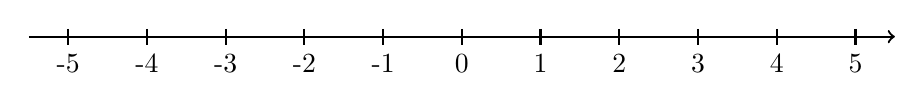
\begin{tikzpicture}
  % Línea principal
  \draw[->, thick] (-5.5,0) -- (5.5,0);

  % Marcas y etiquetas
  \foreach \x in {-5,...,5} {
    \draw[thick] (\x,0.1) -- (\x,-0.1); % marcas
    \node[below] at (\x,-0.1) {\x};     % etiquetas
  }
\end{tikzpicture}
\end{center}

\subsection*{Problem 4}
Graph $-2 \leq x < 4$ on a number line.  

\begin{center}
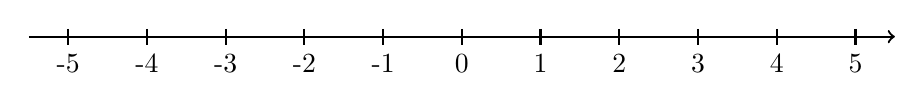
\begin{tikzpicture}
  % Línea principal
  \draw[->, thick] (-5.5,0) -- (5.5,0);

  % Marcas y etiquetas
  \foreach \x in {-5,...,5} {
    \draw[thick] (\x,0.1) -- (\x,-0.1); % marcas
    \node[below] at (\x,-0.1) {\x};     % etiquetas
  }
\end{tikzpicture}
\end{center}

\subsection*{Problem 5}
Graph the inequality: $x$ is greater than or equal to two.  

\begin{center}
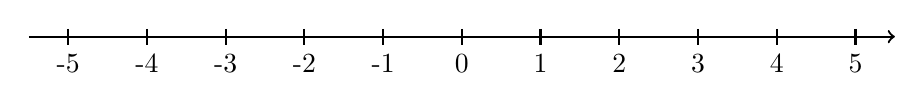
\begin{tikzpicture}
  % Línea principal
  \draw[->, thick] (-5.5,0) -- (5.5,0);

  % Marcas y etiquetas
  \foreach \x in {-5,...,5} {
    \draw[thick] (\x,0.1) -- (\x,-0.1); % marcas
    \node[below] at (\x,-0.1) {\x};     % etiquetas
  }
\end{tikzpicture}
\end{center}

\subsection*{Problem 6}
Solve the linear equation:  
\[
-2(a - 3) = 3(a - 2)
\]

\subsection*{Problem 7}
Solve the following proportion:  
\[
\frac{x}{18} = \frac{4}{36}
\]

\subsection*{Problem 8}
Translate the statement. Let $p$ represent the unknown percent value:  
\textit{278 is what percent of 105?}

\subsection*{Problem 9}
Translate each statement into an equation using \( x \) to represent the unknown value:
\begin{enumerate}[label=(\alph*)]
    \item What percent of 115 is 35?
    \item The number 35 is 15\% of what number?
    \item What is 32\% of 812?
\end{enumerate}


\subsection*{Problem 10}
A car uses 22 gallons of gasoline for a trip of 400 miles.  
How many gallons would be used on a trip of 200 miles?

\subsection*{Problem 11}
Solve the percent equation:  
What number is 25\% of 162?

\subsection*{Problem 12}
Solve the percent equation:  
135 is 250\% of what number?

\subsection*{Problem 13}
Convert the decimal to a percent:  
\[
0.0725
\]

\subsection*{Problem 14}
Convert the percent to a decimal:  
\[
3.72\%
\]

\subsection*{Problem 15}
Draw the graph of a line with an $x$-intercept of 3 that passes through the point $(-3, -2)$.  

\begin{center}
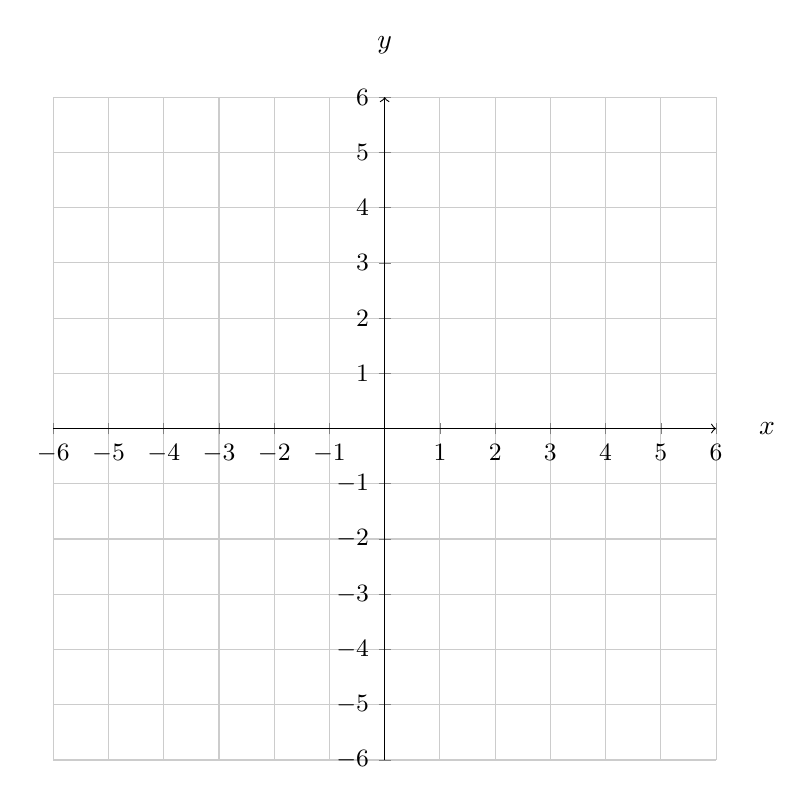
\begin{tikzpicture}
  \begin{axis}[
    axis lines=middle,
    xmin=-6, xmax=6,
    ymin=-6, ymax=6,
    xtick={-6,-5,...,6},
    ytick={-6,-5,...,6},
    grid=both,
    major grid style={line width=0.4pt,draw=black!20},
    width=10cm,
    height=10cm,
    enlargelimits=false,
    axis line style={->},
    ticks=both,
    xlabel={$x$},
    ylabel={$y$},
    every axis x label/.style={at={(ticklabel* cs:1.05)}, anchor=west},
    every axis y label/.style={at={(ticklabel* cs:1.05)}, anchor=south},
    tick label style={font=\small}
  ]
  \end{axis}
\end{tikzpicture}
\end{center}


\subsection*{Problem 16}
Solve the following equation with constants on both sides:  
\[
6x - 8 = 31
\]

\subsection*{Problem 17}
Solve the equation using the Subtraction and Addition Properties of Equality:  
\[
y + 40 = -62
\]

\subsection*{Problem 18}
Subtract:  
\[
-12.53 - 34.34
\]

\newpage
\subsection*{Problem 19}
Round 51.419 to the nearest:
\begin{itemize}
    \item hundredth
    \item tenth
    \item whole number
\end{itemize}

\subsection*{Problem 20}
For a given assignment, the ratio of students who scored higher than 80\% to students who scored lower than 80\% is 16 to 20.  
Write this ratio as a fraction in simplest form.

\end{document}
